\chapter{Requirements Engineering}


\section{Lernziele}

\begin{itemize}
    \item für kleinere Projekte qualitätssichernde Maßnahmen planen und verfolgen können
    \item Tests planen und dokumentieren können
    \item gefundene Fehler geeignet verwalten können
\end{itemize}

\newpage

\section{Einführung}

\begin{tcolorbox}[title={Software Engineering}]
    \textbf{Software Engineering} beschäftigt sich mit der \textbf{systematischen} und \textbf{methodischen} Entwicklung von Software durch \textbf{ingenieurmäßiges Vorgehen}.
\end{tcolorbox}

\noindent
Unter dem Begriff \textbf{Software} wird nicht allein der Programmcode verstanden, sondern alle \textit{Gegenstände}, die zur Softwareentwicklung gehören, wie bspw. auch die \textit{Dokumentation} des Codes für die Entwickler und die eigentliche \textit{Applikation} für den Anwender sowie die \textit{Daten}, die die Anwendung benötigt.\\
$\rightarrow$ \textbf{Software = Code + Dokumente}\\


\noindent
\textbf{Software Engineering} (i.F. \textit{SE}) will durch \textbf{ingenieurmäßiges Vorgehen} (i.F. \textit{IV}) eine wirtschaftlichere Entwicklung von Software gewährleisten.\\
$\rightarrow$ \textbf{Grundlage für IV: finanzielle Interessen stehen hinter der Software Entwicklung (i.F. \textit{SD})}\\

\noindent
\textbf{IV} bedeutet, dass \textbf{SE} auf wissenschaftlicher Basis und kodifizierter\footnote{
\textit{kodifizieren}: Regeln und Prinzipien in einem systematischen Format zusammenfassen und festlegen.
} Erfahrung beruht.\\

\noindent
IV beruht dabei auf Normen, Standards und Regeln:

\begin{itemize}
    \item\textbf{technische Ebene}: bspw. Vorlagen, wie Anforderungen an Software erfasst werden; Normen für Entwürfe von Software.
    \item \textbf{methodische Ebene}: bspw. festgeschriebene Reihenfolge von Tätigkeiten und zu erstellende Produkte für die Entwicklungsarbeit; Kriterien für den Einsatz technischer oder organisatorische Maßnahmen
\end{itemize}\\

\noindent
\textbf{Menschliche Aspekte} sind für den Prozess der SD genauso wichtig wie \textit{technische}: Kommunikation zwischen Kunde und Entwickler ist wichtig, genauso wie die Berücksichtigung menschlicher Bedürfnisse der Kunden und Endanwender, bspw. hinsichtlich intuitiver Bedienung der Software (s.a. Abschnitt~\ref{sec:anforderungen}).
\section{Vorgehen}

\noindent
Das Ermitteln von Anforderungen erfolgt in drei Schritten (s. Abbildung~\ref{fig:requirementsengineering}):

\begin{enumerate}
    \item \textbf{Domänenanalyse}
    \item[] Alle Beteiligten müssen das Umfeld und die Hintergründe des Projektes kennenlernen, wozu auch die Erwartungen
    der Kunden und Anwender an das Produkt und Projekt gehören.\\
    Ein wesentlicher Teil der Analyse ist es, die Domäne und ihre fachlichen Konzepte zu verstehen sowie sich mit dem Vokabular vertraut zu machen, mit dem der Kunde und seine Mitarbeiter im (Berufs- /Anwendungs-)Alltag kommunizieren
    \item \textbf{Vision \& Scope}
    \item[] Wenn sich ein Auftraggeber Gewinn von der Entwicklung einer Software verspricht, formuliert er aus seiner Geschäftsidee Anforderungen, damit das Produkt erfolgreich ist.
    Das wird als \textbf{Geschäftsanforderungen} bezeichnet und schriftlich in Form des \textbf{Vision \& Scope} bzw. \textbf{Lastenheft} dokumentiert.
    Das Dokument beinhaltet das, was vom Produkt zu erwarten ist, damit das Ergebnis des Projektes wirtschaftlich erfolgreich ist.
    \item \textbf{Requirements}
    \item[] Im dritten Schritt werden aus Anwendersicht funktionale und nicht-funktionale Anforderungen zusammengetragen, die \textbf{Requirements}.
    Hierzu zählen bspw. Arbeitsabläufe, die von der Software erledigt werden sollen, oder aber auch Anforderungen an Antwortzeiten, Speicherplatz etc.
\end{enumerate}



\begin{figure}
    \centering
    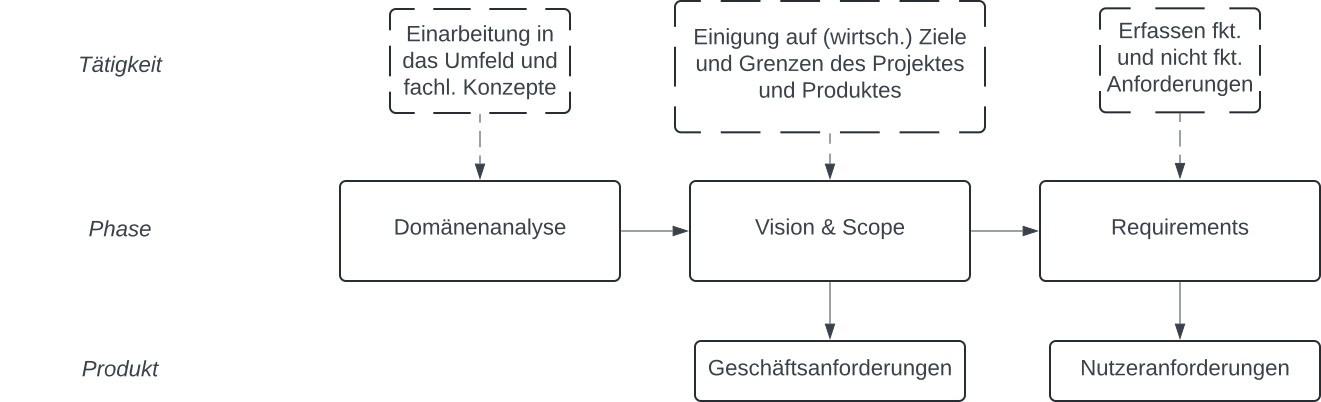
\includegraphics[scale=0.35]{part one/Requirements Engineering/img/requirementsengineering}
    \caption{Phasen des Requirement Engineerings sowie deren Tätigkeiten und Ergebnisse. (Quelle: in Anlehnung an~\cite[84]{Wed09})}
    \label{fig:requirementsengineering}
\end{figure}


\section{Domänenanalyse}

\noindent
Bei der \textbf{Domänenanalyse} eignen sich Entwickler Wissen über die umzusetzende Fachlichkeit an.\\

\noindent
Wissen über die Domäne verspricht ein effektiveres und effizienteres Zusammenarbeiten mit Kunden und Anwendern, da auf einer gemeinsamen Basis kommuniziert werden kann, in der elementare Begriffe und Konzepte der Domende von allen Beteiligten gleich verstanden werden.\\
Dies erleichtert das Vorahnen von Anforderungen bzw. Anpassungen und das Treffen richtiger Entscheidschungen.

\noindent
Domänenwissen veraltet deutlich langsamer als technisches Wissen, weshalb Experten einer speziellen Domäne wertvoll Mitarbeiter sind.\\

\noindent
Domänenwissen kann aus Fachartikeln bzw. Fachbüchern gewonnen werden bzw. in Schulungen oder durch Gespräche mit fachkundigen Mitarbeitern des Kunden bzw. Kollegen.\\
Vevor das gespräch mit Fachexperten genutzt wird, um Detailfragen zu klären, sollte sich der Entwickler zunächst selber einen Überblick über die Fachlichkeit verschaffen, um den Kontext fachbezogener Fragen selber besser einschätzen zu können.\\

\noindent
Nach der Domänenanalyse ist ein Entwickler besser auf seine Aufgabe vorbereitet, und der Informationsaustausch gelingt besser.
Außerdem ist er in der Lage, neuen Mitarbeiter den Einstieg zu erleichtern, wozu solche Informationen auch schriftlich niedergelegt werden sollten.\\
\textit{Wedemann} nennt hierzu folgende Dokumentenarten (vgl.~\cite[42]{Wed09}):

\begin{itemize}
    \item Glossar der wichtigsten Fachbegriffe und deren Bedeutungen
    \item Literaturlisten mit kurzer Bewertung und Inhaltsangabe
    \item Zusammenfassungen von Texten bzw. Auszüge von Texten in Bezug auf das Projekt und das Produkt
    \item Erstellen von Kunden- und Anwenderstrukturen und -organisationen
    \item Auflistung konkurrierender Software
    \item Aufstellung derzeitiger, bereits bekannter Geschäftsprozesse
\end{itemize}
\section{Lastenheft: Vision \& Scope}

Software-Ingenierure helfen Kunden dabei, bei der Entwicklung oder Anpassung von Software einen wirtschaftlichen Nutzen zu erreichen, bspw. eine \textit{erhöhte Produktivität} oder die Einhaltung gesetzlicher Vorschriften.\\
Der Aufwand für die Entwicklungder Softwarelösung muss geringer sein as der voraussichtliche Nutzen, was man unter \textbf{Business Case} zusammenfaßt.

\blockquote[{\cite[11]{Brug09}}]{
    Ein Business Case ist ein Szenario zur betriebswirtschaftlichen Beurteilung einer Investition.
    Auch ein Projekt stellt eine Investition dar und
    muss deshalb seine Vorteilhaftigkeit gegenüber der Geschäftsleitung unter
    Beweis stellen. [...] Ein IT-Projekt ist mit Ausgaben verbunden. Um den Mitteleinsatz zu rechtfertigen, muss dem Management
    aufgezeigt werden, welchen Gegenwert („Return“) es von dem Projekt erwarten kann. Hierzu müssen Annahmen hinsichtlich der voraussichtlichen
    Kosten des Projektes und der mit seinen Ergebnissen erwarteten Ertragsauswirkungen und Kosteneinsparungen getroffen werden.
}

\noindent
Die Ziele des Kunden (\textbf{Vision}) dienen als Voraussetzung für eine Auswahl der Funktionalität für die zu entwickelnde Lösung.\\
Der Projektumfang (\textbf{Scope}) grenzt den Projektumfang ein und gibt Auskunft darüber, was entwickelt werden soll und was nicht.\\
Da der Nutzen für den kunden im Vordergrund steht, muss es sich bei \textbf{Vision \& Scope} um die \textit{Kundensicht} handeln.\\

\noindent
Die \textbf{Stakeholder} - also alle vom Projekt betroffenen Personen - erarbeiten dabei eine gemeinsame Sicht auf die \textit{Zielstellung} und den \textit{Nutzen} des Projektes.\\
Wird auf diesen Schritt verzichtet und keine gemeinsame Sicht erarbeitet, werden mit hoher Wahrscheinlichkeit einige Personen(gruppen) ihre Interessen bei der Anforderungsanalyse oder  Entwicklung nicht vertreten sehen, woraus (tiefgreifende) Anpassungen oder auch die Ablehnung der entwickelten Lösung resultieren kann.\\
Aus diesem Grund ist es eine Frage der Effektivität und der Risikovermeidung, Vision \& Scope \textit{am Anfang} der Entwicklung zu klären (vgl.~\cite[44]{Wed09}).

\noindent
Der Kunde sollte seine Ziele in einem solchen Lastenheft festhalten. \\
Entwickler \ Berater können hier bei der Projektdefinition helfen und auch die Machbarkeit aus technischer Sicht klären.\\

\noindent
Wichtig ist die Klärung von \textit{Kernfragen} in einem solchen Dokument:

\begin{itemize}
    \item Was ist die Vision?
    \item Was soll gemacht werden und was nicht?
    \item Welchen konkreten Nutzen erwartet der Kunden hiervon?
\end{itemize}

\noindent
Der Kurs nutzt hierzu eine Vorlage von \textit{Wiegers}, die wie folgt aufgebaut ist (vgl. \cite[81 ff. sowie 576 ff.]{WJ13}):

\begin{enumerate}
    \item Geschäftsanforderungen
        \begin{enumerate}[label*=\arabic*.]
            \item Hintergrund
            \item Geschäftsmöglichkeit
            \item Geschäftsziele und Erfolgskriterien
            \item Erfordernisse von Kunde oder Markt
            \item Geschäftsrisiken
        \end{enumerate}
    \item Vision der Lösung
        \begin{enumerate}[label*=\arabic*.]
            \item Vision
            \item Wichtigste Features
            \item Annahmen und Abhängigkeiten
        \end{enumerate}
    \item Fokus und Grenzen
        \begin{enumerate}[label*=\arabic*.]
            \item Umfang des ersten Release
            \item Umfang der folgenden Releases
            \item Begrenzung und Ausschlüsse
        \end{enumerate}
    \item Geschäftskontext
        \begin{enumerate}[label*=\arabic*.]
            \item Stakeholder
            \item Projektprioritäten
            \item Technische Anwendungsumgebung
        \end{enumerate}
\end{enumerate}

\subsection*{1. Geschäftsanforderungen}
Dieser Abschnitt stellt dar, \textbf{wie} und \textbf{für wen} umgesetzt werden soll.

\subsubsection*{1.1 Hintergrund}
Enthält eine zusammenfassung über die Hintergründe, die zzu der Entscheidung geführt haben, die Software zu entwickeln.

\subsubsection*{1.2 Geschäftsmöglichkeit}
Für \textbf{kommerzielle Systeme werden} in diesem Abschnitt \textit{Marktlücke} und \textit{Markt} beschrieben, bei \textbf{Invividualentwicklungen} das \textit{Geschäftsproblem} und die zu \textit{verbessernden Geschäftsprozesse}.

\subsubsection*{1.3 Geschäftsziele und Erfolgskriterien}
Die \textbf{wichtigsten Nutzen} des Projektes werden in diesem Abschnitt auf \textit{messbare} Art und Weise zusammengefasst, wie \textit{Marktanteile}, \textit{Umsatzziele}, \textit{Gewinnziele}, \textit{Einhaltung gesetzlicher Vorgaben}, \textit{Ablösung von nicht mehr unterstützter Sofztware} und / oder \textit{Hardware}.

\subsubsection*{1.4 Erfordernisse von Kunde oder Markt}
Die \textbf{Bedürfnisse} des \textbf{Kunden} oder eines \textbf{Nutzers} des Marktsegments werden in diesem Abschnitt beschrieben.

\subsubsection*{1.5 Geschäftsrisiken}
\textbf{Geschäftsrisiken} können sich sowohl für eine Entwicklung als auch für eine Nichtentwicklung ergeben.
Entsprechend werden diese in diesem Abschnitt aufgeführt.

\subsection*{2. Vision der Lösung}
In diesem Abschnitt ist die \textbf{strategische Vision} für die Entwicklung festgehalten, wobei hier weder auf  detaillierte Anforderungen noch auf die Projektplanung eingegangen wird.

\subsubsection*{2.1 Vision}
Enthält eine \textbf{prägnante Beschreibung der Vision}, die den \textbf{langfristigen Nutzen} und das \textbf{Ziel des neuen Produkts} beschreibt.

\subsubsection*{2.2 Wichtigste Features}
\textbf{Wesentliche Features} werden zusammen mit \textbf{eindeutigen Bezeichnern} aufgeführt.

\subsubsection*{2.3 Annahmen und Abhängigkeiten}
Alle \textbf{Annahmen} der \textbf{Stakeholder}, die bei der Erarbeitung von \textbf{Vision \& Scope} geäußert wurden, sind hier festgehalten.\\
Andere Stakeholder werden diesen Annahmen u.U. nicht zustimmen.

\subsubsection*{3. Fokus und Grenzen}

\subsubsection*{3.1 Umfang des ersten Release}
Die \textbf{wichtigsten Features} des \textbf{ersten Release} werden hier aufgeführt, außerdem die \textbf{Qualitätsmerkmale} des ersten Releases.\\
Manche Qualitätsmerkmale wie Performance, GUI-Design können u.U. erst für ein späteres Release wichtig sein.

\subsubsection*{3.2 Umfang der folgenden Releases}
Die \textbf{Features} der \textbf{nochfolgenden Releases} werden hier aufgeführt.

\subsubsection*{3.3 Begrenzung und Ausschlüsse}
Der Abschnitt definiert, was \textbf{zu dem Produkt gehört} und was nicht.\\
Auch Funktionen, die von  solche einer Lösung erwartet werden würden, die aber nicht geplant sind, werden hier aufgeführt.

\subsubsection*{4. Geschäftskontext}

\subsubsection*{4.1 Stakeholder}
Die \textbf{wichtigsten Stakeholder} werden hier aufgeführt, sowie den Nutzen, den diese von dem Projekt haben, ihre Einstellung zu dem Projekt, für sie wesentliche Features sowie Einschränkungen, denen die Stakeholder unterliegen\footnote{
\textit{Einschränkungen} bei \textit{Wiegers}: \textit{constraints}. Ein \textit{constraint} für Vertriebsmitarbeiter könnte bspw. sein, dass diese die Anwendung fast ausschließlich mobil nutzen, oder dass andere Stakeholder (bspw. nicht technisch-affine Mitarbeiter) Schulungen in neu eingeführten Systemen benötigen
}.

\subsubsection*{4.2 Projektprioritäten}
Führt die \textbf{Prioritäten des Projektes} auf, die \textbf{von allen Stakeholdern} unterstützt werden müssen.\\
Nach Möglichkeit sollen hierzu $5$ Kategorien unterschieden werden: \textit{Feature}, \textit{Qualität}, \textit{Termin},
\textit{Kosten}, \textit{Mitarbeiter}. \\
Es kann zudem unterschieden werden zwischen \textit{festen}, \textit{anpassbaren} und \textit{gewählten} Prioritäten.\\

\subsubsection*{4.3 Technische Anwendungsumgebung}
Beschreibt die \textbf{technische Umgebung}, in der die Anwendung laufen soll. also \textit{Hardware}, \textit{Betriebssysteme}, \textit{Netzwerk} usw.\\
Anforderungen an \textbf{Verfügbarkeit} und \textbf{Performance} und \textbf{Sicherheit} haben hier genauso ihren Platz.\\
Außerdem wird festgehalten, ob \textbf{Nutzer} oder \textbf{Hardware} \textbf{räumlich verteilt} sind.
\section{Kontextdiagramme}

\textbf{Kontextdiagramme} liefern eine grafische Übersicht der Systeme in ihrem Kontext.\\
Die Systeme selber werden dabei ohne innere Struktur dargestellt, da diese erst bei \textbf{Architektur} und \textbf{Entwurf} festgelegt wird.\\
Ein Kontextdiagramm zeigt darüber hinaus Schnittstellen zu anderen Systemen oder auch Anwendern und stellt die wichtigsten Anwendungsfälle dar.\\

\noindent
Als Notation für Kontextdiagramme werden i.d.R. \textbf{UML-Use-Case-Diagramme} benutzt, wobei Systeme als Pakete dargestellt werden, bei denen ihr Datenfluss durch Pfeile mit Richtungsangaben dargestellt wird (s. Abbildung~\ref{fig:usecaseexample}).

\begin{figure}
    \centering
    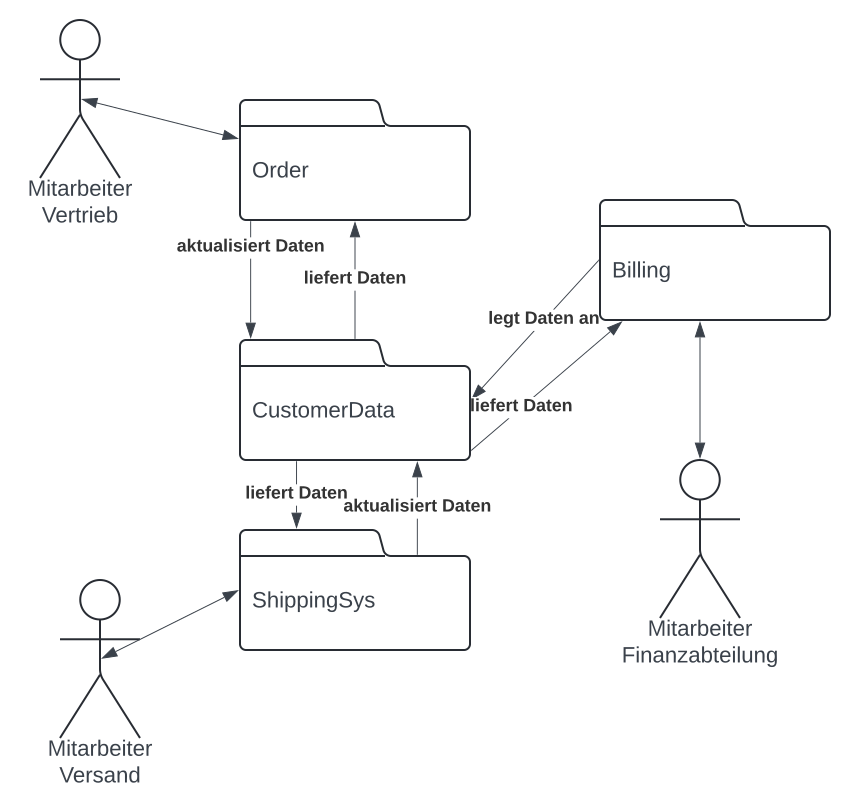
\includegraphics[scale=0.4]{part one/Requirements Engineering/img/usecaseexample}
    \caption{Beispiel für ein Kontextdiagramm. (Quelle: eigene)}
    \label{fig:usecaseexample}
\end{figure}

\section{Typische Probleme und ihre Lösungen}

Eine \textbf{ausführliche} und \textbf{verlässliche Berechnung} ist bei großen Projekten wegen der Auftragssumme Grundvoraussetzung für die Beauftragung einer Entwicklung.\\

\noindent
Deshalb wird i.d.R. zuerst ein \textbf{Vision \& Scope} erstellt und die \textbf{Rentabilität} sorgfältig geprüft.\\

\noindent
Wesentliche Fragen sollten aber auch bei kleineren Projekten geklärt werden, indem auch dort ein Lastenheft erstellt wird - ggfl. reicht hier auch nur eine stichpunkthaltige Zusammenfassung der wesentlichsten Punkte.\\

\noindent
Es sollte bei der Erstellung von \textbf{Vision \& Scope} in jedem Fall darauf geachtet werden, die \textbf{Stakeholder miteinzubeziehen}, damit keine wichtigen Anforderungen übersehen werden.\\

\noindent
In diesem Zusammenhang zeigt sich auch immer wieder, dass verschiedene Mitarbeiter der Kunden sehr unterschiedliche Sichten auf die Aufgaben haben können, was zu \textbf{gegensätzlichen} bzw. \textbf{sich widersprechenden Anforderungen} führen kann.\\
\textit{Bewertung}, \textit{Wichtigkeit} und \textit{Zweckmäßigkeit} einzelner Anforderungen können aufgrund unterschiedlicher Ziele oder Aufgaben divergieren.\\
Hierbei hilft Vision \& Scope, die Anforderungen \textbf{gemeinsam zu erarbeiten} und eine \textbf{gemeinsame Lösung} zu definieren.
Ansonsten könnten Mitarbeiter, die ihre Interessen verletzt sehen, gegen das System \textbf{opponieren} oder es torpedieren (bspw. indem sie keine weiteren Informationen oder nur Fehlinformationen beitragen).\\

\noindent
Wird eine neue Software zur Änderung und / oder Optimierung von Prozessen eingesetzt, kann dies ebenfalls dazu führen, dass \textbf{Mitarbeiter befürchten}, ihre Arbeit nicht mehr in dem Rahmen durchführen zu dürfen, wie sie das bisher getan haben\footnote{oder gar ihren Job zu verlieren}.\\
Um die \textbf{spätere Akzeptanz} zu gewährleisten, sollten auch solche Punkte im Lastenheft mit aufgeführt sein.\\
Spezialisierte \textbf{Organisationsentwickler} können dabei helfen, in einem Diagnose-Prozess zusammen mit den Beteiligten die aktuelle Situation zu untersuchen und bestehende Probleme zu identifizieren, um ein \textbf{gemeinsames Bewusstsein für das Problem} zu schaffen.\\
Sie begleiten außerdem den Soll-Entwurfsprozess, in dem von allen Beteiligten eine gewünschte Zukunft entworfen wird.\\
Diese Prozesse ziehen sich meist durch die gesamte Softwareentwicklung (vgl.~\cite[53]{Wed09}).\\

\noindent
Die Arbeit an Anforderungen hilft auch dem Kunden, eigene Bedürfnisse besser zu verstehen, weshalb sich die \textbf{Sicht auf ein Projekt} im Laufe der Entwicklung \textbf{ändern} kann.\\
Das \textbf{Management} sollte dabei die \textbf{Abweichungen verfolgen} und bei Abweichungen zum Vision \& Scope gemeinsam mit den \textbf{Stakeholdern} dieses \textbf{nochmal überprüfen}.\\
Ansonsten kann die entwickelte Lösung auf Ablehnung stoßen, was Nacharbeiten oder ein Scheitern des Projektes bedeutet.
\section{Anforderungen}\label{sec:anforderungen}

\vspace{5mm}
\begin{tcolorbox}
    Die Entwicklung und Einführung einer Software ist für eine Unternehmen dann erfolgreich, wenn die im Vision \& Scope definierten Ziele in der Praxis erreicht werden, unter Voraussetzung, dass die Endanwender auch tatsächlich mit dem System arbeiten können: Hierzu müssen die Anforderungen der Endanwender unter Berücksichtigung der \textbf{Geschäftsanforderungen} des Kunden erfüllt sein (vgl.\cite[54]{Wed09}).
\end{tcolorbox}
\vspace{5mm}

\subsubsection*{Anforderungen Kunde \& Anwender}
Nicht nur die Anforderungen des Kunden sind ein wesentliches Kriterium für die Umsetzung des Projektes, sondern auch die Wünsche und Bedürfnisse der Endanwender müssen gesammelt und dokumentiert werden.\\

\subsubsection*{Vorgehen}
Um die Anforderungen auf geeignete Weise schriftlich festzuhalten, was auch als Grundlage für die Vertragsgestaltung sowie zur weiteren Planung dient und Mißverständnissen vorbeugt, kann man folgendes Vorgehen wählen:

\begin{itemize}
    \item Identifizierung der Endanwender.
    \item Auswahl von Stellvertretern der Stakeholdern.
    \item Gemeinsame Erarbeitung der Anforderungen mit den Stellvertretern.
    \item Dokumentation der \textbf{nicht-funktionalen} und \textbf{funktionalen Anforderungen} als User-Storys, Anwendungsfälle, Regeln oder Eventtabellen.
\end{itemize}


\subsection{Die Stimme des Kunden}
\subsubsection*{Anforderungen werden mit dem Anwender erarbeitet}
Oftmals sind Kunden und Endanwender nicht in der Lage, Bedürfnisse strukturiert und widerspruchsfrei zu äußern, außerdem sind Anforderungen und Lösungsvorschläge verschiedener Anwender nicht immer miteinander vereinbar oder widersprechen sich oder dem erstellen \textbf{Vision \& Scope}, manchmal liefern Anwender auch (wissentlich) Falschinformationen.\\

\noindent
Eine unreflektierte Umsetzung der Anforderungen wäre also ein Fehler, weshalb es Aufgabe des Entwicklers ist, gemeinsam mit dem Kunden die Anforderungen zu bearbeiten.

\subsection*{Nutzerklassen}
Anwender unterscheiden sich (im Bezug auf das neue System) hinsichtlich

\begin{itemize}
    \item Häufigkeit der Nutzung
    \item Erfahrung mit dem Umfeld
    \item ihrer Tätigkeiten und damit der benötigten Features
    \item Zugriffsrechte
    \item Computerexpertise
\end{itemize}

\noindent
Basierend darauf ist es möglich, Nutzer in unterschiedliche \textbf{Nutzerklassen} einzuteilen.\\
Hierbei ist es auch möglich, dass ``Nutzer`` keine Person beschreiben, sondern andere Systeme, die über entsprechende Schnittstellen mit dem geplanten System interagieren werden.

\subsection*{Stellvertreter}
Damit die verschiedenen Nutzerklassen berücksichtigt werden können, sollten konkrete Personen die jeweiligen Klassen vertreten: Diese definieren die Anforderungen und stimmen diese mit den Stellvertretern anderer Klassen ab.\\
Ausreichende Entscheidungsbefugnisse der Stellvertreter verhindern unnötige Rückfragen/-versicherungen.\\
Stellvertreter können auch dabei helfen, Testfälle für das System zu definieren.

\subsection*{Sind alle Bedürfnisse vertreten?}
Ein Problem bei diesem Ansatz ist, dass die Stellvertreter wirklich die Interessen der Nutzerklassen vertreten, was bspw. über Feedbackschleifen  (unter Einbeziehung der tatsächlichen Nutzer) sichergestellt werden kann.\\
Hierzu können Vertreter des Anforderungsteams gewählt werden, um als Vermittler zu fungieren: Dies kann als Teil des \textit{Informationsprozesses} gesehen werden, der eine \textit {Organisationsentwicklung} begleitet\footnote{s.a. \cite[53]{Wed09}, wo erwähnt wird, wie ein \textit{Diagnoseprozess} von Organisationsentwicklern organisiert wird, um bestehende Probleme und Befürchtungen in der Organisation bei der Einführung neuer Software/Prozesse zu untersuchen}.

\subsection*{Techniken}
Unterschiedliche Quellen, wie bspw. Interviews mit Mitarbeitern, in denen Wünsche und Bedürfnisse in Hinsicht auf die neue Software - oder auch Unzufriedenheit mit der bestehenden Lösung - geäußert werden, können als Quelle für Anforderungen dienen.\\

\noindent
Die genaue Untersuchung und Analyse von bestehender Software (bspw. Formulare zum Anlegen von Daten für benötigte Geschäftsprozesse), aber auch das Begleiten der Anwender beim Einsatz der Bestandslösung kann dabei helfen, die Anforderungen zu verstehen bzw. auszumachen\footnote{
Siehe hierzu auch Aufgabe 4.8 in \cite{Wed09}.
}.
Vor allem der letzte Fall kann auch dabei helfen, Vertrauen zwischen Mitarbeitern und Entwicklern herzustellen.\\

\noindent
Auch die Analyse bestehender konkurrierender Softwareprodukte im Hinblick auf Stärken und Schwächen kann hilfreich sein.

\subsection*{Klassifizierung der Angaben der Nutzer}
Die Angaben der Anwender können systematisch sortiert werden.
Es eignet sich bspw. eine Einteilung in

\begin{itemize}
    \item \textbf{Nicht-funktionale Anforderungen} (Performance, Verfügbarkeit, Nutzerfreundlichkeit etc.)
    \item \textbf{Anwendungsfälle und User-Storys} zur Beschreibung funktionaler Anforderungen
    \item \textbf{Regeln} die die verschiedenen \textbf{Geschäftsobjekte} erfüllen müssen
    \item \textbf{Interface-Beschreibungen} Beschreibung der Schnittstellen zu anderen Systemen, vorgegebenen Dateiformaten oder der Hardware.
    Das GUI als Mensch/Maschine-Schnittstelle wird i.d.R. erst bei der Analyse entworfen.
    \item \textbf{Datendefinitionen}: Informationen, in welchem Format bestimmte Daten vorliegen müssen.
    Wird bei der Anforderungsphase im sogenannten \textbf{Datadictionary} (s. Abschnitt \ref{sec:datadictionary-und-mengengerust}) gesammelt.
    \item \textbf{Lösungsideen} der Mitarbeiter, wie bestimmte Prozesse vereinfacht / verbessert abgebildet werden können.
    Hier sollten \textit{alle} Lösungsideen erfasst werden, auch solche, die ggf. als unmöglich umsetzbar/ widersprüchlich erscheinen
\end{itemize}


\section{Nicht-funktionale Anforderungen}\label{sec:nicht-funktionale-anforderungen}

\noindent
\textbf{Nicht-funktionale Anforderungen} werden in \textbf{Qualitätsanforderungen} und \textbf{Randbedingungen} unterschieden:

\begin{itemize}
    \item \textbf{Qualitätsanforderungen} beschreiben die Qualität oder Eignung eines Systems (Performance, Benutzerfreundlichkeit, \ldots)
    \item \textbf{Randbedingungen} beschreiben technische Anforderungen (Programmiersprache, Framework, \ldots) oder organisatorische Anforderungen (Budget, Deadlines, \ldots)
\end{itemize}

\noindent
Auch nicht-funktionale Anforderungen verursachen Aufwand, da sie in allen Phasen mitberücksichtigt werden müssen.\\
Es ist deshalb nötig, alle nicht-funktionalen Anforderungen zu priorisieren, und sich gemeinsam mit Kunde und Anwendern auf die notwendigsten zu einigen.\\
Gute Praxis ist es, die Qualitätsmerkmale genau zu definieren.

\subsection*{Nicht-funktionale Anforderungen sind entscheidend}
Nicht-funktionale Anforderungen sind insb. entscheidend für die Systemarchitektur.\\
Es muss zumindest \textit{eine} Systemarchitektur vorhanden sein, die die fundamentalen Anforderungen (Erreichbarkeit, Antwortzeiten, Funktionalität) abdeckt.

\subsection*{Systematik der Qualitätsanforderungen}
Vorgefertigte Kategorien und Typen von Qualitätsmerkmalen können bei der Erfassung von Qualitätsanforderungen helden, die Übersicht zu bewahren und keine wichtige Anforderung zu übersehen\footnote{man nennt dies \textit{systematische Aufstellungen} bzw. \textit{Qualitätssysteme}}.\\

\noindent
Die im Kurs verwendete Systematik folgt dem Standard \textbf{IEEE 1061-1998}:

\blockquote[{\url{https://standards.ieee.org/ieee/1061/1549/}\footnote{abgerufen 01.04.2024}}]{
    This IEEE Standards product is part of the family on Software Engineering. A methodology for establishing quality requirements and identifying, implementing, analyzing, and validating the process and product software quality metrics is defined. The methodology spans the entire software life cycle.
}

\noindent
Es existieren u.a. folgende Kategorien:

\begin{itemize}
    \item \textbf{Verfügbarkeit (Availability)}: geplante Betriebszeit, während der das System vollständig nutzbar ist (formal beschrieben durch Verhältnis tatsächlicher Uptime / geplanter Uptime).
    Als Ausfallzeit werden i.d.R. nur ungeplante Ausfälle gezählt, aber nicht die Wartungsfenster.
    \item \textbf{Effizienz (Efficiency)}: Maß, wie gut ein System vorhandene Systemresourcen (Speicher, Prozessorleistung) nutzt.
    Nötig, wenn mehrere Programme auf dieselben Systemressourcen zugreifen muss, oder wenn Erweiterungen geplant sind
    \item \textbf{Erweiterbarkeit (Flexibility / Extensibility)}: beschreibt, wie leicht neue Funktionalität in das System eingebaut werden kann, um es zu erweitert\footnote{
        bspw. können \textbf{Functional Points} verwendet werden, um die Komplexität eines Dialogs im UI zu messen. Jedes \textit{control} erhält hier einen Wert, die Summe ergibt die ``Komplexität``
    }.
    \item \textbf{Wartbarkeit}: Änderbarkeit des Systems aus technischer Sicht.
    Hiermit ist vor allem die\textit{Änderung existierender Funktionalität} gemeint, im Gegensatz zu \textbf{Erweiterbarkeit}, die die Erweiterung des Funktionsumfangs beschreibt
    \item \textbf{Integrität (Integrity)}: Sicherheit des Systems, bspw. gegen unberechtigte Zugriffe
    \item \textbf{Interoperabilität (Interoperability)}: wie leicht das System mit anderen Systemen kommunizieren oder Daten austauschen kann (bspw. Export in andere Formate, Schnittstellen zu externen Systemen, \ldots)
    \item \textbf{Zuverlässigkeit (Reliability)}: Durchschnittliche Zeit oder durchschnittliche Anzahl an Operationen, während der ein System fehlerfrei arbeitet
    \item \textbf{Robustheit (Robustness)}: Das Verhalten des Systems unter fehlerhaften (Rand-)Bedingungen (Falscheingaben, Hardwarefehler, \ldots)
    \item \textbf{Benutzbarkeit (Usability)}: Bedienbarkeit des Programms, bspw. Ergonomie, Barrierefreiheit, wie lange bestimmte Prozesschritte benötigen, bis sie von einem erfahrenen / unerfahrenen Anwender durchgeführt wurden, \ldots
    \item \textbf{Portabilität (Portability)}: Aufwand, eine Software auf ein anderes OS / eine andere Hardware zu portieren (bspw. \textit{mobile})
    \item \textbf{Wiederverwendbarkeit (Reusability)}: Anforderung an Wiederverwendbarkeit einzelner Komponenten / Subsysteme in anderen Systemen; bedeutet i.d.R. zusätzlichen Aufwand durch Absprachen der involvierten Teams
    \item \textbf{Testbarkeit (Testability)}: Software muss so konstruiert sein, dass Testverfahren durchgeführt werden können (bspw. in der Industrie, wenn Testverfahren vorgeschrieben sind). \textbf{Testbarkeit} entspricht zumeist auch \textbf{Wartbarkeit}, da eine Software gut wartbar ist, wenn sie testbar ist (Probleme mit Änderungen können über Testfälle abgefangen werden), und umgekehrt gut testbar, wenn sie wartbar ist (bspw. lassen sich neue Funktionen leicht integrieren und gut testen, wenn eine \textit{lose Kopplung} und \textit{höhe Kohäsion} im System vorhanden ist).
    \item \textbf{Performance}: Antwortzeit bei Anfragen an das System.
    Faustregel: Systeme mit direkter Nutzeraktion sollten 1 sek als Antwortzeit nicht überschreiten; in manchen Umgebungen sind Antwortzeiten nicht garantierbar (Internet), im Embedded-Bereich müssen sie garantiert werden können (vgl.~\cite[62]{Wed09}).
    Vorhersehbare Kriterien wie Im-/Export großer Datenmengen über das Internet müssen berücksichtigt werden, da sich solche Gegebenheiten auf den Entwurf/die Architektur auswirken können (bspw. wegen Komprimierungsverfahren).
\end{itemize}


\subsection*{Probleme ergeben sich, wenn Wichtiges fehlt}
Eine genaue Auswahl, Definition und Priorisierung hilft allen Stakeholdern, sich auf gemeinsame und realistische Ziele zu einigen.\\
Dabei sollte darauf geachtet werden, auch die Anforderungen mit zu erfassen, die nicht Teil eines Standards sind, weil alle geäußerten Anforderungen erheblichen Einfluss auf das Produkt haben können.


\subsection{Technische Randbedingung}\label{subsec:technische-randbedingung}
\textbf{Randbedingungen} sind eine weitere wichtige Kategorie von nicht-funktionalen Anforderungen.

\vspace{2mm}
\begin{tcolorbox}
    \blockquote[{\cite[65, Hervorhebung eigene]{Wed09}}]{
        Bei \textbf{Randbedingungen} handelt es sich um Vorgaben vom Kunden, nicht um die Vorstellung der Softwareentwickler.
    }
\end{tcolorbox}
\vspace{2mm}

\noindent
Unterschieden wird hierbei zwischen \textbf{technischen} und \textbf{organisatorischen} Randbedingungen.\\

\noindent
Randbedingungen sind nicht priorisierbar, aber es kann angegeben werden, ob diese \textit{fest} oder \textit{anpassbar} sind.

\begin{itemize}
    \item \textbf{Technische Randbedingungen} definieren die einzusetzenden technischen Komponenten, wie bspw.
        \begin{itemize}
            \item Hardware-Infrastruktur
            \item Software-Infrastruktur
            \item Programmiersprachen
            \item Frameworks
        \end{itemize}
    \item \textbf{Organisatorische Randbedingungen} sind Vorgaben, die die Organisation des Projektes betreffen, wie bspw.
    \begin{itemize}
        \item Termine
        \item Dokumentationsvorgaben
        \item Vorgaben zur Vorgehensweise
        \item Vorgaben zu Tests oder Abnahmeprozessen
    \end{itemize}
\end{itemize}

\noindent
Organisatorische Randbedingungen können im einzelnen auf unterschiedliche Aspekte des Projektes Auswirkungen haben (QS, Implementierung, Projektorganisation).\\

\noindent
Es kann mitunter herausfordernd sein, zwischen eigenen Ideen und den Kundenanforderungen zu unterscheiden, was aber wichtig ist, da ``Randbedingungen Einschränkungen für mögliche Lösungen darstellen und damit entscheidende Auswirkungen auf die gesamte Tätigkeit haben`` (\cite[65]{Wed09}).
\section{Funktionale Anforderungen}

\vspace{5mm}
\begin{tcolorbox}
    \textbf{Funktionale Anforderungen} definieren, welche Funktionen eines zu entwickelnden Systems von Endanwendern oder anderen Systemen benutzt werden können (\cite[66]{Wed09}).
\end{tcolorbox}
\vspace{5mm}

\noindent
Ein weit verbreiteter Ansatz zur Erarbeitung von Anforderungen ist die Erfassung von \textbf{Anwendungsfällen} (\textit{Use Case}), oder auch von \textbf{User Stories}.\\

\noindent
Die Verfahren können gleichzeitig eingesetzt werden, da sind unterschiedlich detailliert sind und andere Perspektiven beleuchten.

\subsection*{User Story}

\textbf{User Stories} beschreiben in ein bis zwei Sätzen, wie ein Endanwender mit dem System arbeiten möchte, bspw. ``Der Vertrieb bezieht aus dem System die Wiedervorlageliste und protokolliert die durchgeführten Gespräche`` (s. a. Aufgabe 4.13. in \cite{Wed09}).\\

\noindent
Eine \textbf{User Story} ist aufgrund der fehlenden Details als eine Art \textbf{Merkhilfe} für Stakeholder und Entwickler zu verstehen, und nicht als formale Beschreibung eines Prozesses; idealerweise werden die Storys von den Stakeholdern erstellt.\\

\noindent
User Stories sind dazu geeignet, ``die Welt des Kunden zu verstehen``\footnote{
\textit{Wedemann} verweist hier auf \textit{Beck}, s.~\cite[66]{Wed09}
}.\\

\noindent
Es kann durchaus passieren, dass sich User Stories widersprechen, wenn mehrere unterschiedliche Stakeholder die Storys erstellen.\\

\noindent
Auf eine \textit{exakte und detaillierte} Beschreibung der einzelnen Storys wird \textit{verzichtet}, da davon ausgegangen wird, dass die Stellvertreter der Endanwender jederzeit erreichbar sind.\\

\noindent
\textbf{Story Cards} (Karteikarten) werden verwendet, um die Storys zu notieren.\\
I.d.R. werden sie für Planungszwecke mit einer Nummer, sowie Kennungen für Priorität und Aufwand versehen.


\begin{itemize}
    \item \textbf{Vorteile}
        \begin{itemize}
            \item hilfreich für die direkte Arbeit mit den Endanwendern: Beschreibung, was mit dem System gemacht werden soll, hilft dem Endanwender, über seine Wünsche zu reflektieren, und dem Entwickler, die Bedürfnisse des Kunden zu verstehen
        \end{itemize}
    \item \textbf{Nachteile}
        \begin{itemize}
            \item schwierig, wenn Stakeholder nicht (dauernd) anwesend oder nicht erreichbar sind, da die knappe schriftliche Form zu vage ist, womit auch eine Dokumentation fehlt
            \item Formalisierung (wie in Anwendungsfällen) würde es den Stakeholdern und Endanwendern möglich machen, nichts zu vergessen und bei komplizierten Sachverhalten den Überblick zu behalten
        \end{itemize}
\end{itemize}

\subsection*{Anwendungsfall}
\blockquote[{\cite[67, Hervorhebung eigene]{Wed09}}]{Ein \textbf{Anwendungsfall} beschreibt, wie Nutzer mit einem System in einer abgeschlossenen, ununterbrochenen Folge arbeiten, um ein fachliches Ziel zu verwirklichen.}

\noindent
Die Abläufe sollten für die Beschreibung als Anwendungsfälle nicht zu komplex sein.\\

\noindent
Man unterscheidet i.d.R. zwischen zwei Typen von Anwendungsfällen: \textbf{Grundlegende Anwendungsfälle} (\textit{Essential Use Case}) und \textbf{traditionelle Anwendungsfälle} (\textit{System Use Case}).

\subsubsection*{Grundlegender Anwendungsfall (Geschäftsvorfall)}
Ein \textbf{Grundlegender Anwendungsfall} beschreibt \textit{unter vollständigem Verzicht} auf Details der Technik oder der späteren Umsetzung, wie der Endnutzer mit dem System umgeht und wie das System darauf reagieren soll (vgl.~\cite[68]{Wed09}).\\

\noindent
Der Anwender ist hierbei in der Regel der \textbf{Akteur}, externe Systeme oder Hardware können als auch als \textit{Akteure} gesehen werden.\\
Das umzusetzende System selber ist nie ein Akteur.

\subsubsection*{Traditioneller Anwendungsfall (Systemanwendungsfall)}
\textbf{Traditionelle Anwendundgsfälle} können deutlich detaillierter als grundlegende Anwendungsfälle sein und \textit{Details der Implementierung berücksichtigen}.\\
Sie unterscheiden sich außerdem im Format zu den grundlegenden Anwendungsfällen und können unterschiedlich detailliert ausfallen.\\

\noindent
Ansatz zur Erstellung:

\begin{enumerate}
    \item Anwendungsfall \texctit{high-level} erstellen (Überschrift, grobe Formulierung der einzelnen Schritte)
    \item Anwendungsfall \textit{informell} erstellen (grundlegender Ablauf)
    \item Anwendungsfall \textit{formell} ausprägen
\end{enumerate}


\subsubsection*{Probleme mit formellen Anwendungsfällen}
Für die detaillierte bzw. formelle Ausprägung von Anwendungsfällen eignen sich eher Werkzeuge und Hilfsmittel, die während der Analysephase verwendet werden, wie \textbf{Aktivitätsdiagramme} der Anwendungsfälle, \textbf{Entwürfe} und \textbf{Ablaufdiagramme} der Benutzeroberfläche, oder das \textbf{Domänenmodell}.\\
Mit diesen Werkzeugen kann dann auch das Zusammenspiel mehrerer Anwendungsfälle modelliert werden, wie \textit{Wedemann} feststellt (vgl.~\cite[71]{Wed09}).\\

\noindent
Insgesamt entstehen viele Dokumente: Je umfangreicher das Projekt, desto häufiger müssen diese Dokumente geändert werden, was zusätzlichen Aufwand bedeutet.\\
Man sollte deshalb abwägen, welche Dokumente für den Einmalgebrauch bestimmt sind und welche auch für die zukünftige Dokumentation und Planung geeignet sind.

\subsection*{UML Use Case-Diagramm}
Bei größeren Systemen, in denen Stakeholder und Entwickler gemeinsam viele Anwendungsfäll entwickeln, werden \textbf{Use Case-Diagramme} verwendet, die durch die \textit{Unifield Modeling Language} \textbf{UML} standardisiert sind.\\
\section{Ereignistabellen}
Anforderungen als \textbf{Ereignisse} zu beschreiben eignet sich insb. dann, wenn für Geräte entwickelt wird.\\

\noindent
Als \textit{Ereignis} wird hier eine Änderung oder Aktivität verstanden, die eine Antwort der Software auslöst.


\begin{table}
[htbp]
    \centering
    \begin{tabular}{|l|l|l|l|}
        \hline
        \textbf{Nr} & \textbf{Ereignis} & \textbf{Systemzustand} & \textbf{Antwort}   \\
        \hline
        1 & \textit{play} & \textit{gestoppt} & \textit{spielt}   \\
        \hline
        2 & \textit{play} & \textit{spielt} & \textit{stop}   \\
        \hline
        3 & \textit{weiter} & \textit{gestoppt} & \textit{nächstes Lied}   \\
        \hline
        4 & \textit{weiter} & \textit{spielt} & \textit{nächstes Lied, spielt}   \\
        \hline
    \end{tabular}
    \caption{Beispiel für eine Ereignistabelle für einen mp3-Player (Quelle: eigene)}\label{tab:ereignistabelle}
\end{table}


\section{Regeln}
\textbf{Geschäftsregeln} (\textit{Business Rules}), die in der Software implementiert werden müssen, verstehen sich als zugrundeliegende Regeln von (Geschäfts-)Prozessen.\\
Die Einhaltung dieser Regeln erhöht die Zuverlässigkeit der Anwendung und die Qualität der Daten.\\

\noindent
Geschäftsregeln können in folgende Typen eingeteilt werden:

\begin{itemize}
    \item \textbf{Randbedingungen (Constraint)} beschränken, was Nutzer tun dürfen (Stichwörter \textit{muss}, \textit{darf nicht}, \textit{nur})
    \item \textbf{Aktionsauslöser (Action Enabler)} beschrieben, was nach Auslösung eines Ereignisses passiert (\textit{wenn \ldots, dann} [Aktion])
    \item \textbf{Wissenserzeuger (Inference)} erzeugen neues Wissen, wenn eine Bedingung zutrifft (\textit{wenn \ldots, dann} [neues Wissen])
    \item \textbf{Berechnung (Computation)}: Vorschriften zur Berechnung mit Formeln oder Algorithmen
\end{itemize}

\noindent
Regeln sollten in einer Art \textit{Regelbuch} festgehalten werden.\\
Stakeholder und Entwickler haben dadurch die gleiche Sicht auf alle Regeln.\\
Folgende Spalten sind sinnvoll:

\begin{itemize}
    \item Nummer der Regel
    \item Beschreibung der Regel
    \item Typ der Regel
    \item Dynamik der Regel\footnote{\textit{statisch} oder \textit{dynamisch}, also ändert sich die Regel, oder bleibt sie unverändert?}
    \item Quelle\footnote{aus welchem Geschäftsbereich stammt die Regel?}
\end{itemize}
\section{Datadictionary und Mengengerüst}\label{sec:datadictionary-und-mengengerust}
In einem \textbf{Datadictionary} wird festgehalten, in welchem Format welche Daten verarbeitet werden.\\

\noindent
Über solch ein zentrales Dokument kann erreicht werden, dass unterschiedliche Anwendungsteile einheitliche Datenformate nutzen.\\

\noindent
Zur Datendefinition gehören:

\begin{itemize}
    \item Typ (\textit{String}, \textit{Integer}, \textit{Aufzählungen}, \ldots)
    \item Format (bspw. kalendarische Datumsformate)
    \item ggf. die Einheit
    \item andere \textit{Daten} bei zusammengesetzten Datentypen (bspw. bei Adressen)
\end{itemize}

\noindent
Zu beachten ist, dass es sich bei dem Datadictionary um ein \textbf{vorläufiges Dokument} handelt: Es dient dazu, Informationen, die während der Anforderungsphase gesammelt wurden, systematisch zu sammeln.\\
$\rightarrow$ die endgültige Datendefinition erfolgt erst in der Analysephase, weil dann erst genügend Informationen zusammengetragen wurden.

\vspace{5mm}
\begin{tcolorbox}
    Das Datadictionary ist als strukturierte Merkhilfe zu verstehen.
\end{tcolorbox}
\vspace{5mm}

\subsection{Mengengerüst}
Das \textbf{Mengengerüst} beschreibt die zu erwartende Anzahl der Daten\footnote{Kundendatensätze, Adressdatensätze, \ldots} als wichtiges Kriterium, da sich damit festgehaltene Kennzahlen direkt auf die Architektur bzw. Datenhaltung (Datenbanksysteme) auswirken kann.\\

\noindent
\textit{Wedemann} merkt an, dass es sich hierbei streng genommen um eine \textit{nicht-funktionale} Anforderung handelt, aber nicht-funktionale Anforderungen meist globaler gefasst sind als ein detailliertes Mengengerüst (\cite[76]{Wed09}).
\section{Pflichtenheft}

\noindent
Ein übliches Vorgehen ist es, die nach \textit{Vision \& Scope} entwickelten Dokumente
\begin{itemize}
    \item nicht-funktionale Anforderungen
    \item funktionale Anforderungen (Anwendungsfälle)
    \item Regeln (Geschäftsregeln)
    \item Datadictionaries und Mengengerüste
\end{itemize}

in einzelnen Dokumenten über ein Dokumentenmanagementsystem zur Verfügung zu stellen.\\
Dadurch können einzelne Dokumente separat bearbeitet und versioniert werden.\\

\noindent
Wird allerdings nach dem \textbf{Wasserfallmodell} gearbeitet, werden die Ergebnisse i.d.R. in einem durchgehenden Dokument zur Verfügung gestellt, dem \textbf{Pflichtenheft}.\\

Der Kurs nutzt hierzu die Gliederung nach dem Vorbild von \textbf{IEEE 830}\footnote{
mit Modifikationen  von \textit{Wiegers} aus \cite[190 ff.]{WJ13}
}:

\blockquote[{\url{https://standards.ieee.org/ieee/830/1222/}\footnote{abgerufen 02.04.2024}}]{
    The content and qualities of a good software requirements specification (SRS) are described and several sample SRS outlines are presented. This recommended practice is aimed at specifying requirements of software to be developed but also can be applied to assist in the selection of in-house and commercial software products.
}

\noindent
Das Pflichtenheft kann dabei wie folgt aufgebaut sein (s.a. \cite[190 ff.]{WJ13}):

\subsection*{1. Einführung}
Aufbau des Pflichtenhefts, Hinweise zur Verwendung.

\subsubsection*{1.1 Zweck des Dokuments}
Welches System beschrieben wird, Verweis auf Vision \& Scope.

\subsubsection*{1.2 Konventionen des Dokuments}
Typographische / formale Konventionen, Priorisierungen etc.

\subsubsection*{1.3 Zielgruppe}
Welche Leser mit dem Dokument bedient werden, Hinweise auf die für die jeweilige Lesergruppe essenziellen Abschnitte.

\subsubsection*{1.4 Produktfokus}
Verweis auf Vision \& Scope. Beschreibt das Pflichtenheft den Release einer Software, wird hier der Fokus des Release aufgeführt.

\subsubsection*{1.5 Referenzen}
Andere Dokumente, die in dem Pflichtenheft referenziert werden, sind hier aufgeführt, inkl. Angaben zu den Quellen.


\subsection*{2. Beschreibung}


\subsubsection*{2.1 Produkt-Perspektiven}
Verweis auf Vision \& Scope. Beschreibung des Kontexts und des Ursprungs des Systems.

\subsubsection*{2.2 Produkt-Funktionen}
Auflistung der wichtigsten Features und Funktionen. Verweis auf Vision \& Scope und Kontextdiagramm.

\subsubsection*{2.3 Anwenderklassen}
Nennung aller Klassen von Endanwendern.

\subsubsection*{2.4 Betriebsumgebung}
Die Hardware-Plattform, das Betriebssystem, die Datenbank, \ldots mit denen das System arbeiten soll.

\subsubsection*{2.5 Randbedingungen für Entwurf und Umsetzung}
Weitere und noch nicht genannte Randbedingungen, wie Programmiersprache, Frameworks, \ldots

\subsubsection*{2.6 Anwenderdokumentation}
Aufführung der zu liefernden Anwenderdokumentation.

\subsubsection*{2.7 Annahmen und Abhängigkeiten}
Beschreibung, welche Annahmen bei der Erstellung getroffen wurden, welche Abhängikeiten es von externen Faktoren gab.


\subsection*{3. System Features}

\subsubsection*{3.x Anwendungsfall x}
Beschreibung der einzelnen Anwendungsfälle, die mit der Software abgedeckt werden. \textit{Wiegers} unterteilt in \cite[194]{WJ13} weiter in \textit{3.x.1 Beschreibung} und \textit{3.x.2 Funktionale Anforderungen}

\subsection*{4. Externe Schnittstellen}

\subsubsection*{4.1 Nutzerschnittstellen}
Standards oder Vorschriften zum Layout (GUI).
Keine Dialogentwürfe, da diese Teil der Analysephase sind.

\subsubsection*{4.2 Hardwareschnittstellen}

\subsubsection*{4.3 Softwareschnittstellen}

\subsubsection*{4.4 Kommunikationsschnittstellen}
Protokolle und/oder Anwendungen, die verwendet werden sollen

\subsection*{5. Weitere nicht-funktionale Anwendungen}

\subsubsection*{5.1 Performance}
\subsubsection*{5.2 Sicherheit}
\subsubsection*{5.3 Qualität}
Weitere, noch nicht genannte Qualitätsanforderungen.

\subsection*{6. Weitere Anforderungen}
Geschäftsregeln, Internationalisierung etc.


\subsection{Vor- und Nachteile}
Als Vorteil einer solchen Gliederung der Informationen in \textit{ein} Dokument ist sicherlich die Konsistenz des Formats, in dem die Anforderungen zur Verfügung gestellt werden müssen: Durch die Vorgabe der Gliederung ist es eher unwahrscheinlich, dass einige (wichtige) Teile vergessen werden.\\

\noindent
Sind allerdings mehrere Autoren an der Erstellung des Dokumentes beteiligt, müssen entsprechende Maßnahmen zur Verwaltung getroffen werden (bspw. VCS).\\
Da in der Gliederung immer wieder auf Vision \& Scope verwiesen wird, ist eine Abgrenzung zu diesen eher unklar.\\
Wichtige Anforderungen wie Geschäftsregeln werden in der Vorlage nur am Ende erwähnt (vgl.\cite[79]{Wed09}).\\

\noindent
\textit{Wedemann} empfiehlt in \cite[80]{Wed09} - im Gegensatz zu Vision \& Scope - auf die Zusammenfassung in einem Dokument zu verzichten und stattdessen einzelne Dokumente zu verwenden, die auf die Problemstellung zugeschnitten sind.


\newpage
\section{Zusammenfassung}

\begin{itemize}
    \item Anforderungen lassen sich bei Projekten vorab nicht genügend festlegen.
    \item Fehlt im Team die Erfahrung oder werden neue Technologien eingesetzt, ist ein ausgereifter Entwurf nicht machbar.
    \item Bei großen Projekten würde man unter diesen Voraussetzungen mit dem Wasserfallmodell nicht flexibel genug sein,
    um auf Änderungen reagieren zu können.
    \item Aus diesem Grund gibt es alternative Modelle, die eingesetzt werden können:
        \begin{itemize}
            \item \textbf{inkrementell}: Aufteilung der Anforderungen, so dass Teilsysteme umgesetzt und an den Kunden ausgeliefert werden können
            Die Teilsysteme werden sequentiell bearbeitet.
            \item \textbf{iterativ}: In Iterationen wird das Projekt in Zeitabschnitte unterteilt, in denen die Anforderungen umgesetzt werden; entsprechend dem Spiralmodell zunächst die risikoreichsten.
            Vorhergehende Ergebnisse werden in darauffolgenden Iterationen weiterbearbeitet.
            Ein bekanntes iteratives Modell ist \textit{RUP}, bei dem einzelne Phasen Ergebnis-Artefakte liefern, wie Anwendungsfälle oder Klassendiagramme.
            \item \textbf{nebenläufig}: Die Aufgaben werden aufgeteilt in parallel (oder nacheinander) bearbeitbare Aufgaben, die dann von den Mitarbeitern umgesetzt werden.
        \end{itemize}
    \item Die genannten Modelle werden häufig nicht isoliert betrachtet, sondern je nach Projekt auch kombiniert, insb. bei dem \textbf{agilen Vorgehen}.
\end{itemize}
\newpage

%\section{Lösungsvorschläge}

\subsection{Aufgabe 4.1}

s. Abbildung~\ref{fig:requirementsengineering}.


\subsection{Aufgabe 4.2}

Eine Domänenanalyse sollte durchgeführt werden, damit Hintergründe und (geschäftl.) Umfeld des Projektes und des zu erstellenden Produktes klar sind.\\
Eine Einarbeitung in fachliche Konzepte und eine Aneignung der Sprache / des Vokabulars / der Fachbegriffe erleichtert zudem die Kommunikation in den initialen und nachfolgenden Phasen des Projektes und der Projektplanung.\\
Kenntnisse über die Fachlichkeit ermöglicht es zudem, wichtige Informationen zu verstehen und sich diese für zukünftige Diskussionen und Entwürfe zu merken.

\subsection{Aufgabe 4.3}
Fachliteratur ermöglicht es, sich einen Überblick über die Grundlagen und Konzepte des Projektes und des zu erstellenden Produktes zu verschaffen.\\
Gespräche mit Kollegen können dazu beitragen, das Verständnis für bestimmte Themen zu schärfen, entweder in der Diskussion über eine bestimmte Thematik, oder - wenn der Kollege bereits
eingearbeitet ist - häufig festgestellte Unklarheiten aus dem Weg zu räumen und Mißverständnisse gegenüber bestimmter Themen zu klären.\\
Erst dann sollte im Gespräch mit dem Kunden bzw. Fachexperten über Spezifikationen oder Details gesprochen werden, damit man nicht allzu häufig aufgrund fehlendem Fachwissens später rückfragen muss.\\
Darüberhinaus kann mit einer soliden Grundlage an Fachwissen auch Funktionalität und Bedürfnisse vorhergeahnt werden, außerdem kann Funktionalität im Vorhinein berücksichtigt werden, die nur auf Basis des Fachwissens als selbstverständlich erscheint.

\subsection{Aufgabe 4.4}
s. Tabelle~\ref{tab:stakeholder}.

\subsection{Aufgabe 4.5}
\textbf{Für} die Kunden und Mitarbeiter des Straßenbahnunternehmens XYZ sowie die Kunden der DB, \\
\textbf{die} Auskünfte zu Fahrplänen, Störungen und Preisen im vom XYZ bedienten Nahverkehr benötigen,\\
\textbf{ist} die webbasierte Softwarelösung ABC eine Auskunftsplattform,\\
\textbf{die} diese Informationen über das Internet bzw. die DB bereitstellt.\\
\textbf{Anders als} mit schriftlichen Plänen oder Aushängen ist es \textbf{mit Produkt} ABC möglich, diese Informationen von überall stets aktuell beziehen zu können sowie diese Informationen anderen Systemen zur Verfügung zu stellen.\\
Dies verspricht eine höhere Nutzerzufriedenheit sowie mehr Kunden.


\subsection{Aufgabe 4.6}

s. Abbildung~\ref{fig:aufgabe4-6}.

\begin{figure}
    \centering
    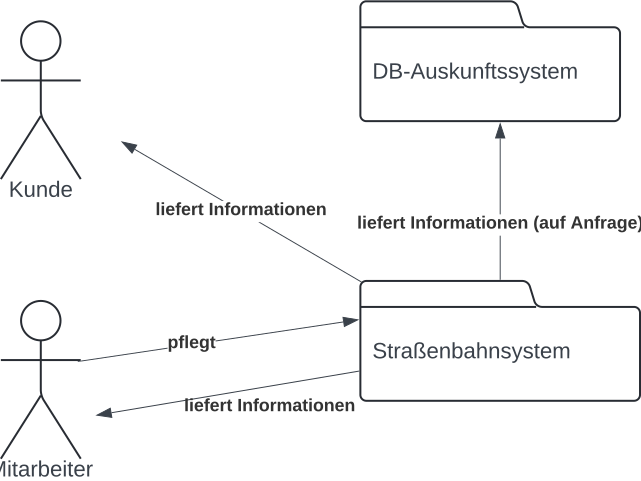
\includegraphics[scale=0.35]{chapters/Requirements Engineering/img/aufgabe4.6}
    \caption{}
    \label{fig:aufgabe4-6}
\end{figure}


%\newpage
